\documentclass[12pt]{report}
\usepackage{indentfirst}
\usepackage{graphicx}
\usepackage{float}
\usepackage{amsmath}
\usepackage{tkz-graph}
\usepackage{pgfplots}
\usepackage[a4paper, total={7in, 10in}]{geometry}

\graphicspath{ {./Images/} }

\setlength{\parskip}{0.2em}
\renewcommand{\baselinestretch}{1.0}

\begin{document}

\title{\Huge{\textbf{FEUPBook}} \\ Relatório BDAD 2019/2020 \\ \Large{2MIEIC04}}
\author{Eduardo Correia \\ \texttt{up201806433} \and
	    Ricardo Fontão \\  \texttt{up201806317} \and
        João Diogo \\ \texttt{up201806779}}
\date{\today}

\begin{figure}[b] % Bottom of page
    \centering
    
\includegraphics[width=0.8\textwidth]{feup-logo}
\end{figure}

\maketitle

\tableofcontents

\chapter{Introdução}

O nosso projeto consiste numa rede social denominada \textit{FEUPBook} (inspirado pela já existente rede social,  \textit{Facebook}). Nesta, utilizadores poderão criar uma conta pessoal para falar uns com os outros, através da troca de mensagens de texto e ver diversas publicações do seu interesse no seu \textit{feed} (a página inicial), bem como organizar \textbf{eventos}, juntarem-se em \textbf{grupos} ou edificar uma \textbf{página} dedicada a algum assunto em particular.

\chapter{Especificação} 

\section{Publicador}

Esta classe tem como função identificar quem são os elementos que podem realizar publicações, registar que publicações efetuaram e atribuir-lhes um \underline{nome}.

\subsection{Utilizador}

Esta classe representa um \textbf{membro} da rede social. Este possui um \underline{id} único para o identificar (correspondente ao último campo do \textit{url} do seu perfil. \par

Um utilizador possui ainda vários outros dados pessoais (que o utilizador pode optar por não preencher por motivos de privacidade): \underline{número de telemóvel}, \underline{data de nascimento}, \underline{género} (masculino ou feminino), morada (\underline{rua} e \underline{localização}). \par

Um \textbf{utilizador}, por norma, terá diversas \textbf{amizades} com outros utilizadores, para que possa aceder aos conteúdos do seu perfil, conversar mais facilmente com ele e ver as publicações no seu feed.\par

Para esse efeito, terá de enviar um pedido de amizade ao outro, o qual pode ser \textbf{aceite} ou não. Se for aceite, a ligação \textbf{pedido de amizade} deixa de existir e passa a ser uma ligação de \textbf{amizade}. Se for rejeitada, essa ligação deixa de existir sem ser substituída por nenhuma outra a um novo \textbf{pedido de amizade} surgir por parte de um dos dois utilizadores.

Tanto uma \textbf{amizade} como um \textbf{pedido de amizade} registam a \underline{data} em que foram efetuados.

\subsection{Página}

Esta classe representa uma \textbf{página} na nossa rede social. \par

Esta tem também associada a si várias publicações. \par

Os utilizadores relacionam-se com um página na medida em que um deles é o seu \underline{administrador} (normalmente correspondente ao criador da página, mas este cargo pode ser transferido) e possui vários \underline{seguidores}, utilizadores que colocaram gosto na página e vêm as publicações no feed.

Tem um \underline{utilizador} que é o seu administrador e pode ter muitos seguidores(utilizadores).

\section{Conversa}

Numa \textbf{rede social} é indispensável a capacidade de os utilizadores conversarem entre si, como tal estes podem agregar-se numa \underline{conversa} (que possui no mínimo 2 utilizadores). \par

Uma \textbf{conversa} é composta por diversas \underline{mensagens}. \par

Ainda neste contexto, cada utilizador pode possuir uma \underline{alcunha} própria.

\section{Multimédia}

A rede social do nosso projeto possui a capacidade de partilhar ficheiros \textbf{multimédia}, quer seja através de mensagens ou publicações e dividem-se essencialmente em três \textbf{categorias}, áudio, imagem e vídeo. Cada ficheiro destes possui um \underline{título}, correspondente ao seu nome em memória, bem como um \underline{url} que indica a localização do ficheiro para lhe aceder. \par

É possível, no entanto, enviar qualquer tipo de ficheiros, não só áudio, imagem ou vídeo, porém se a sua extensão não corresponder a nenhum deste tipo de ficheiros, será enviado como um ficheiro binário que o utilizador pode descarregar. \par

Existe ainda um limite máximo do tamanho ficheiro que o utilizador pode enviar e é de 25 MB. \par

Tanto o \textbf{áudio} como \textbf{vídeo} possuem um \underline{comprimento} da sua duração em segundos.

\section{Atividade}

Vários conteúdos na rede social terão \textbf{reações} por parte dos \textbf{utilizadores}, como tal, esta classe tem o objetivo de agregar esses mesmos conteúdos e manter o registo das reações que possuem. \par

Cada um desses conteúdos possui \underline{texto} a acompanhá-los e a \underline{data} em que foram efetuados.

\subsection{Publicação}

Não só com \textbf{mensagens} é possível comunicar na rede social, mas também com \textbf{publicações}. Possuem o benefício de não serem tão privadas (não precisam de ter um destinatário em particular, ficando publicadas no perfil do \textbf{publicador} em questão que seja o autor da \textbf{publicação}). \par

Esta pode ser composta por multimédia (áudio, foto ou vídeo) de tipos iguais ou diferentes. \par

Agrega ainda vários comentários feitos por utilizadores que pretendam demonstrar a sua opinião em relação à mesma. \par

\subsection{Mensagem}

Uma \textbf{mensagem} é o modo como os utilizadores comunicam numa \underline{conversa}. \par

Pode ser uma mensagem de texto, a partilha de um ficheiro multimédia ou ambos, ou seja, um utilizador pode enviar um ficheiro multimédia com descrição (texto), sem descrição, ou só uma mensagem de texto. \par

\subsection{Comentário}

Um \textbf{comentário} é feito por um \textbf{utilizador} a uma \textbf{publicação} como modo de iniciar uma discussão sobre a publicação ou simplesmente realizar algum tipo de observação/denotação. \par

\section{Reação}

Um utilizador nem sempre tem de se manifestar com mensagens ou comentários, podendo optar por simplesmente deixar uma \textbf{Reação}. Para tal, terá a opção de escolher uma das seguintes \textbf{reações}.

\begin{figure}[H]
    \centering
    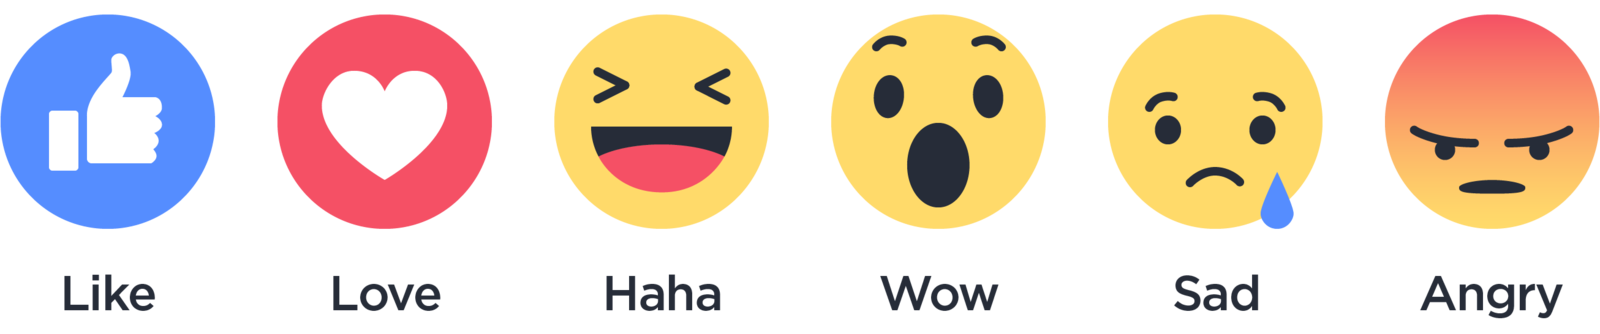
\includegraphics[width=\textwidth]{reactions}
\end{figure}

\section{Evento}

Se um \textbf{utilizador} desejar, pode criar um \textbf{evento} para marcar um \textbf{acontecimento} relevante e convidar outros utilizadores a participarem no mesmo. \par

Um \textbf{evento} possui um \underline{nome} que o identifica, bem como uma breve \underline{descrição} do que se trata e, possivelmente, o local onde se realiza,r e a \underline{data} da sua realização.

Por definição, a reação padrão será o \textit{like}. \par

Um \textbf{utilizador} apenas pode reagir com uma das possíveis reações a um post ou comentários, mas estes podem ter reações de vários utilizadores, inclusive dos seus autores.

\subsection{Grupo}

Um grupo possui como função agregar diversos utilizadores com um interesse em comum. Um utilizador fazendo parte de um grupo, está habilitado a fazer uma publicação, estando esta visível para os restantes membros do grupo. Um grupo tem um utilizador como administrador.

\chapter{Modelo concetual}

\begin{figure}[h!]
    \centering
    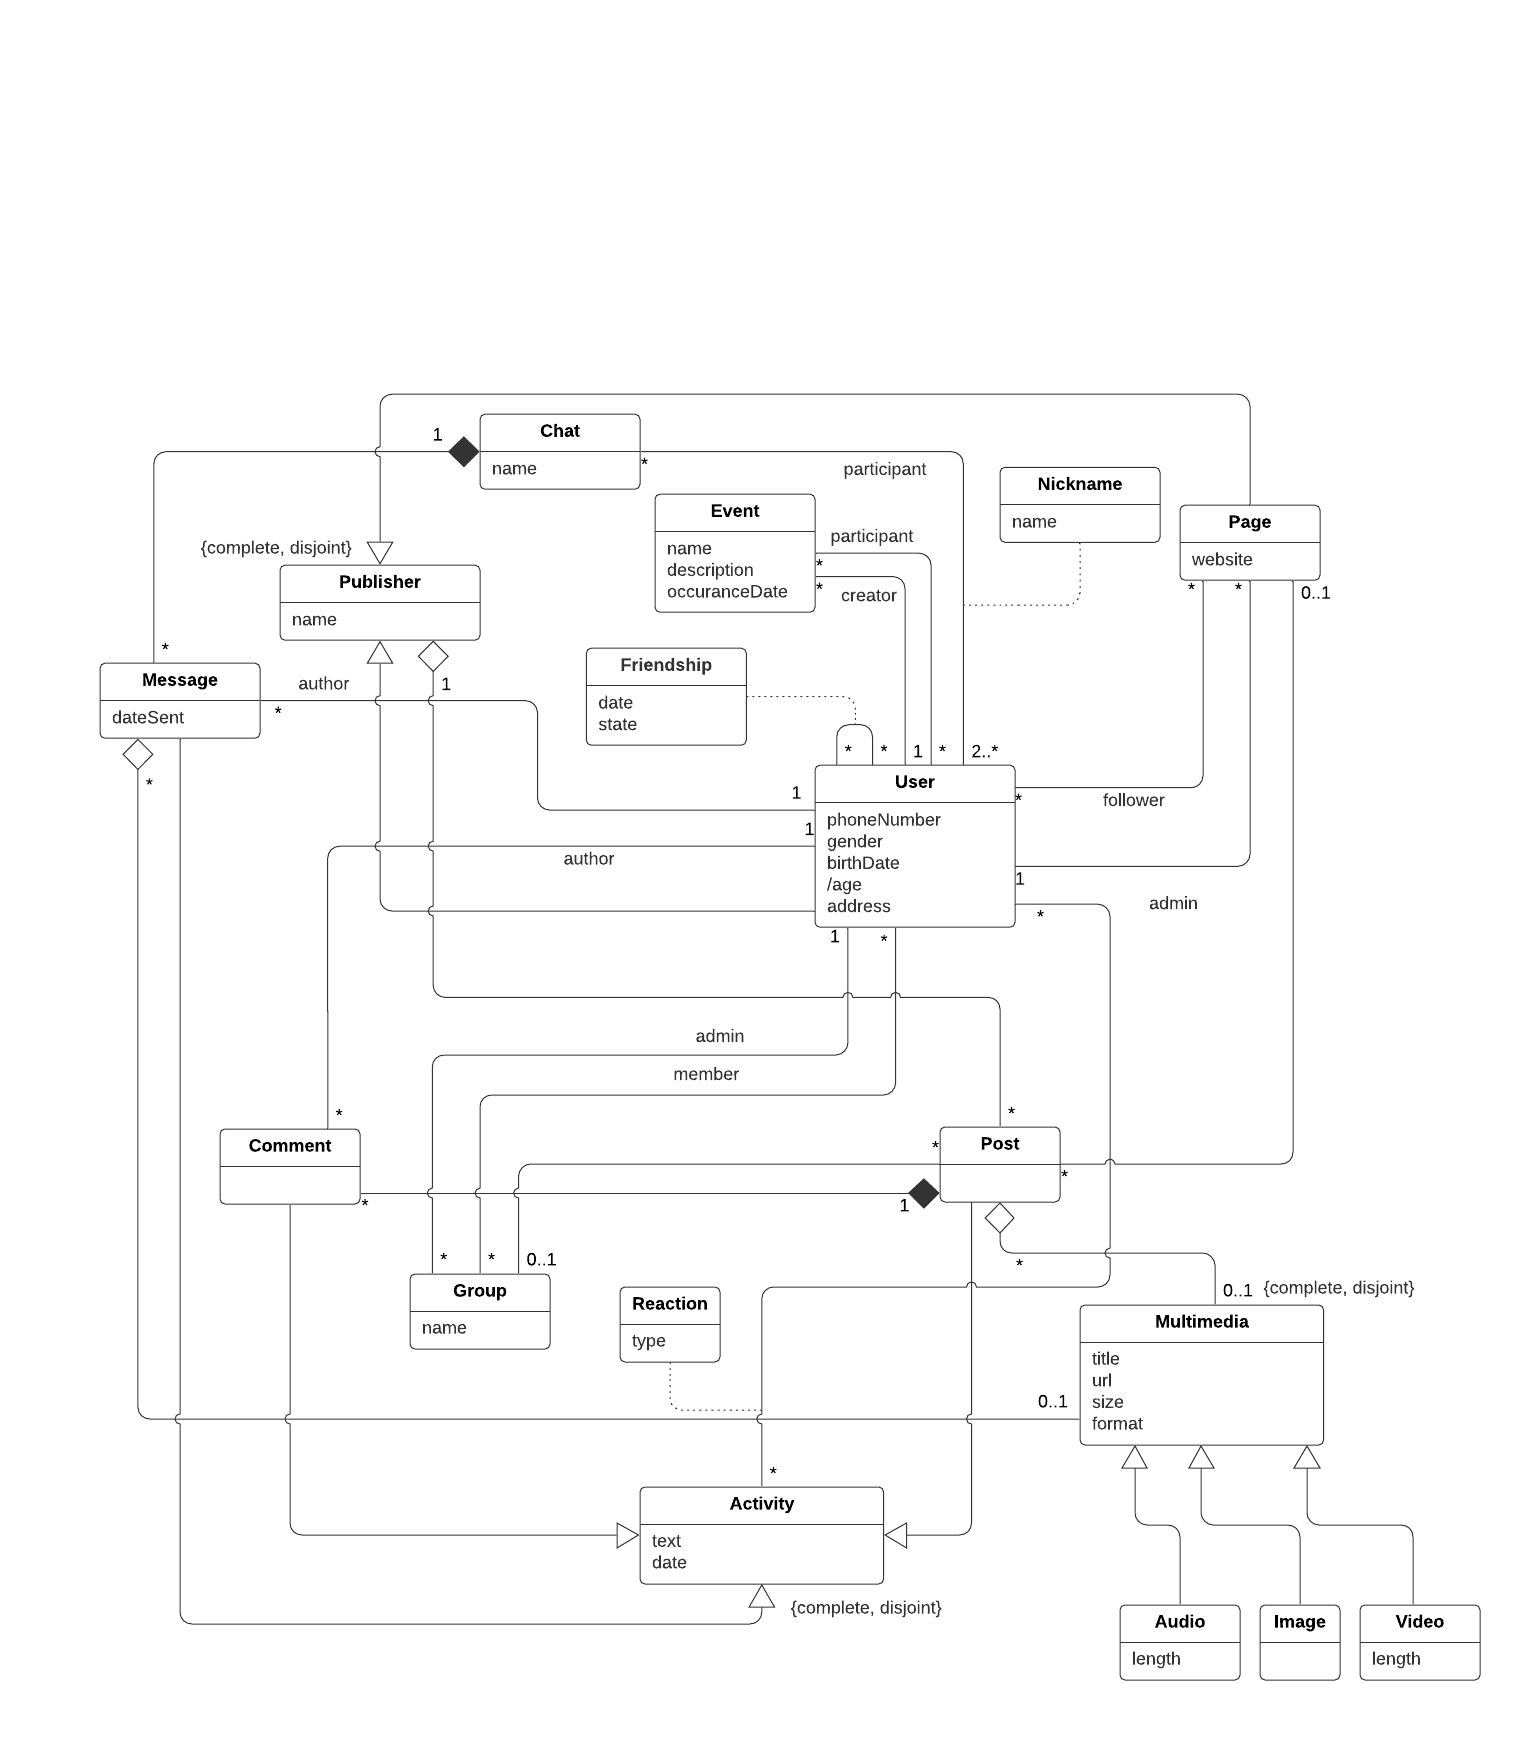
\includegraphics[width=0.8\textwidth]{diagram}
\end{figure}

\chapter{Modelo relacional}

\section{Dependências funcionais}

\textbf{Publisher}(\underline{publisherID}, name)

publisherID $\rightarrow$ name

\vspace{2mm}

\textbf{User}(\underline{userID} $\rightarrow$ Publisher, phoneNumber, gender, birthDate, age, address)

userID $\rightarrow$ phoneNumber, gender, birthDate, age, address

birthDate $\rightarrow$ age

\vspace{2mm}

\textbf{Friendship}(\underline{senderID} $\rightarrow$ User, \underline{receiverID} $\rightarrow$ User, state, date)

senderID, receiverID $\rightarrow$ state, date

\vspace{2mm}

\textbf{Page}(\underline{pageID} $\rightarrow$ Publisher, website, adminID $\rightarrow$ User)

pageID $\rightarrow$ website, adminID

\vspace{2mm}

\textbf{PageFollower}(\underline{followerID} $\rightarrow$ User, pageID)

\vspace{2mm}

\textbf{Group}(\underline{groupID}, name, adminID $\rightarrow$ User)

groupID $\rightarrow$ name, adminID

\vspace{2mm}

\textbf{GroupMember}(\underline{memberID} $\rightarrow$ User, \underline{groupID} $\rightarrow$ Group)

\vspace{2mm}

\textbf{Chat}(\underline{chatID}, name)

chatID $\rightarrow$ name

\vspace{2mm}

\textbf{ChatParticipant}(\underline{participantID} $\rightarrow$ User, chatID $\rightarrow$ Chat, nickname)

participantID, chatID $\rightarrow$ nickname

\vspace{2mm}

\textbf{Multimedia}(\underline{multimediaID}, title, uri, size, format, length)

multimediaID $\rightarrow$ title, uri, size, format, length

uri $\rightarrow$ title, size, format, length

\vspace{2mm}

\textbf{Activity}(\underline{activityID}, text, date)

activityID $\rightarrow$ text, date

\vspace{2mm}

\textbf{Message}(\underline{messageID} $\rightarrow$ Activity, dateSent, multimediaID $\rightarrow$ Multimedia, authorID $\rightarrow$ User, chatID $\rightarrow$ Chat)

messageID $\rightarrow$ dateSent, multimediaID, authorID, chatID

\vspace{2mm}

\textbf{Post}(\underline{postID} $\rightarrow$ Activity, publisherID $\rightarrow$ Publisher, multimediaID $\rightarrow$ Multimedia, pageID $\rightarrow$ Page, groupID $\rightarrow$ Group)

postID $\rightarrow$ publisherID, multimediaID, pageID, groupID

\vspace{2mm}

\textbf{Comment}(\underline{commentID} $\rightarrow$ Activity, authorID $\rightarrow$ User, postID $\rightarrow$ Post)

commentID $\rightarrow$ authorID, postID

\vspace{2mm}

\textbf{Reaction}(\underline{activityID} $\rightarrow$ Activity, \underline{userID} $\rightarrow$ User, type)

activityID, userID $\rightarrow$ type

\vspace{2mm}

\textbf{Event}(\underline{eventID}, name, description, occurenceDate, creatorID $\rightarrow$ User)

eventID $\rightarrow$ name, description, occurenceDate, creatorID

\vspace{2mm}

\textbf{EventParticipant}(\underline{participantID} $\rightarrow$ User, \underline{eventID} $\rightarrow$ Event)

\pagebreak

\section{Análise Forma Normal}

De acordo com o modelo relacional apresentado, todas as relações respeitam a forma normal de Boyce-Codd e,  consequentemente, a 3ª forma normal com a exceção da Relação User. \par
Em birthDate $\rightarrow$ age o elemento que se encontra do lado esquerdo da relação (birthDate) não é uma chave, constitundo deste modo uma violação à BCNF. No entanto, o lado direito da relação apenas é constituído por atributos primos fazendo com que respeite a 3ª forma normal, a qual exige que os atributos do lado esquerdo sejam chaves ou que o lado direito da relação seja apenas contituído por atributos primos. \par
Uma possível solução para este problema seria decompor User do seguinte modo:

\begin{itemize}
    \item User1(birthDate, age)
    birthDate $\rightarrow$ age
    \item User2(id, birthDate, phoneNumber, gender, address)
\end{itemize}

Quanto às restantes relações, uma vez que do lado esquerdo das dependências funcionais se encontram chaves primárias é possível concluir que respeitam a forma normal de Boyce-Codd, e como a 3ª forma normal é um 'super set' desta última também a irão respeitar.

\chapter{Restrições}

\section{Publisher}

\begin{itemize}
    \item \textit{publisherID} é a primary key (key restriction, PRIMARY KEY);
    \item \textit{name} é o nome do Publicador e não pode ser nulo (NOT NULL).
\end{itemize}

\section{User}

\begin{itemize}
    \item \textit{userID} é primary key (key restriction, PRIMARY KEY), é foreign key (referential integrity, FOREIGN KEY) e não pode ser igual a nenhum atributo \textit{pageID} de \textit{Page}.
    \item \textit{phoneNumber} é único a para cada utilizador (UNIQUE);
    \item \textit{gender} apenas pode ter os valores ‘M’ (masculino) e ‘F’(feminino) (CHECK);
    \item \textit{birthDate} não pode ter valores nulos (NOT NULL) e tem que originar uma idade superior a 13 anos (CHECK NOW() - birthDate / 365 $>$ 13)
\end{itemize}

\section{Page}

\begin{itemize}
    \item \textit{pageID} é a primary key (key restriction, PRIMARY KEY), é foreign key (referential integrity, FOREIGN KEY) e não pode ser igual a nenhum atríbuto idUtilizador de Utilizador.
\end{itemize}

\section{ChatParticipant}

\begin{itemize}
    \item (\textit{participantID}, \textit{chatID}) é a primary key (key restriction, PRIMARY KEY) and is a foreign key (referential integrity, FOREIGN KEY).
\end{itemize}

\section{Friendship}

\begin{itemize}
    \item (\textit{senderID}, \textit{receiverID}) é a primary key (key restriction, PRIMARY KEY), é foreign key (referential integrity, FOREIGN KEY) e têm que ser distintos;
    \item \textit{date} corresponde à data do envio do pedido de amizade CHECK(julianday(date) $\leq$ julianday('now')), tem de ser anterior ao momento atual e não pode ter valor nulo (NOT NULL);
    \item \textit{state} corresponde ao estado atual do pedido de amizade e apenas pode possuir os valores 1 (aceite), 2 (pendente) e 3 (rejeitada) (CHECK).
\end{itemize}

\section{EventParticipant}

\begin{itemize}
    \item (\textit{participantID}, \textit{eventID}) é a primary key (key restriction, PRIMARY KEY), é foreign key (referential integrity, FOREIGN KEY).
\end{itemize}

\section{PageFollower}

\begin{itemize}
    \item (\textit{followerID}, \textit{pageID}) é a primary key (key restriction, PRIMARY KEY), é foreign key (referential integrity, FOREIGN KEY).
\end{itemize}

\section{GroupMember}

\begin{itemize}
    \item (\textit{memberID}, \textit{groupID}) é a primary key (key restriction, PRIMARY KEY), é foreign key (referential integrity, FOREIGN KEY).
\end{itemize}

\section{Group}

\begin{itemize}
    \item \textit{groupID} é a primary key (key restriction, PRIMARY KEY);
    \item \textit{name} corresponde ao nome do grupo e não pode ter valor nulo (NOT NULL);
    \item \textit{adminID} é foreign key (referential integrity, FOREIGN KEY).
\end{itemize}

\section{Event}

\begin{itemize}
    \item \textit{eventID} é a primary key (key restriction, PRIMARY KEY);
    \item \textit{name}  corresponde ao \textit{name} do evento e não pode ter valor nulo (NOT NULL);
    \item descrição  corresponde à descrição do evento e não pode ter valor nulo (NOT NULL);
    \item \textit{occurenceDate} corresponde à data em que o evento se realiza e não pode ter valor nulo (NOT NULL);
    \item \textit{creatorID} é foreign key (referential integrity, FOREIGN KEY).
\end{itemize}

\section{Multimedia}

\begin{itemize}
    \item \textit{multimediaID} é primary key (key restriction, PRIMARY KEY);
    \item \textit{size} só pode tomar valores inteiros positivos (CHECK);
    \item \textit{type} pode tomar os seguintes valores: ".mp3", ".jpg", ".png", ".wav", ".mp4"... (CHECK).
    \item \textit{length} só pode tomar valores inteiros positivos (CHECK).
\end{itemize}

\section{Reaction}

\begin{itemize}
    \item \textit{activityID} é primary key (key restriction, PRIMARY KEY) e foreign key (referential integrity, FOREIGN KEY);
    \item \textit{userID} é foreign key (referential integrity, FOREIGN KEY);
    \item \textit{type} representa as formas que a reação pode tomar e pode ter os valores 1, 2, 3, 4, 5 ou 6, correspondentes às reações da figura da secção 2.5 por ordem (CHECK).
\end{itemize}

\section{Comment}

\begin{itemize}
    \item \textit{commentID} é primary key (key restriction, PRIMARY KEY) e foreign key (referential integrity, FOREIGN KEY);
    \item \textit{authorID} é foreign key (referential integrity, FOREIGN KEY);
    \item \textit{postID} é foreign key (referential integrity, FOREIGN KEY).
\end{itemize}

\section{Post}

\begin{itemize}
    \item \textit{postID} é primary key (key restriction, PRIMARY KEY) e foreign key (referential integrity, FOREIGN KEY);
    \item \textit{publisherID}, \textit{multimediaID}, \textit{pageID} e \textit{groupID} são foreign keys (referential integrity, FOREIGN KEY).
\end{itemize}
    
\section{Message}

\begin{itemize}
    \item \textit{messageID} é primary key (key restriction, PRIMARY KEY) e foreign key (referential integrity, FOREIGN KEY);
    \item \textit{multimediaID}, \textit{authorID} e \textit{chatID} é foreign key (referential integrity, FOREIGN KEY);
    \item \textit{dateSent} corresponde à data de envio de uma mensagem e não pode ter valor nulo (NOT NULL).
\end{itemize}

\section{Activity}

\begin{itemize}
    \item \textit{activityID} é primary key (key restriction, PRIMARY KEY);
    \item \textit{date} correponde à data em que a atividade foi realizada. (tem de ser antes do momento presente)
\end{itemize}

\section{Chat}

\begin{itemize}
    \item \textit{chatID} é primary key (key restriction, PRIMARY KEY);
    \item \textit{name} correponde ao nome da conversa e não pode ser nulo (NOT NULL).
\end{itemize}

\chapter{Interrogações}

\section{Publicação com o maior número de likes}

Numa rede social, é comum o fenómeno de existirem publicações virais que arrecadam um número consideravelmente grande de gostos em pouco tempo e, portanto, rapidamente se tornam populares. \par

Daí o propósito desta interrogação que permite obter a publicação mais popular da rede social, ou seja, a que recebeu o maior número de gostos. 

\section{Reação mais comum por utilizador}

Esta interrogação permite obter a reação mais comum de cada utilizador de modo a traçar o seu "perfil". \par

Por exemplo, um utilizador que reage muitas vezes com o \textit{smile} de riso será mais "brincalhão", enquanto que um que faça muitas reações com a carinha triste será mais "melancólico".

\section{Média do tamanho dos ficheiros multimédia enviados por hora}

Frequentemente os utilizadores da rede social trocaram mensagens com elementos multimédia entre si, quer seja para enviar fotos, vídeos, mensagens áudio... \par

Logo, existirá um grande fluxo de dados e como tal, procurou-se calcular essa métrica atráves do rácio MBs / Hora.

\section{Número de mensagens trocadas por cada utilizador em conversas com mais de dois participantes}

Em conversas de grupo com 3 ou mais utilizadores, haverão sempre utilizadores mais ativos do que outros. \par

Alguns serão os autores da maioria das mensagens da conversa, enquanto que outros apenas lerão essas mensagens e raramente irão participar com as suas mensagens. \par
Assim sendo, é possível obter os dados necessários para um estudo estatístico em que se analisaria a participação de cada utilizador, numa conversa de grupo, através desta Interrogação.

\section{Recomendação de amigos}

Numa rede social, os utilizadores desejarão manter os seus amigos por perto, no entanto, poderá ser complicado procurar por todos eles ou até mesmo verificar se já possuem ou não conta no FEUPBook. \par

Para facilitar esse processo, é possível indicar para cada utilizador uma recomendação de amigo, ou seja, uma pessoa que é provável que ele conheça, mas que ainda não é amigo dela. \par

Para se obter essa recomendação, verificou-se, para cada utilizador, qual era a pessoa que possuía o maior número de amigos em comum com os amigos desse utilizador, mas que não era amigo dele.

\section{Utilizadores que são administradores de uma página e de um grupo com o mesmo nome dessa página}

Em princípio, grandes páginas terão um grupo associado à mesma, onde os utilizadores poderão falar sobre os assuntos relativos a esse entidade. \par

Como tal, será de esperar que, por vezes, o administrador do grupo será o mesmo que criara a página e, como tal, será uma pessoa de relevância nesse meio, como por exemplo, o \textit{social media manager} de uma empresa importante que possui tanto uma página, como um grupo.

\section{Número de comentários feitos por dia, no último mês antes de um evento, que se referem ao mesmo}

Com o aproximar de um evento importante (como por exemplo, as Olimpíadas ou o Campenato Europeu de Futebol), deverá haver um aumento progressivo do número de comentários referentes a esse mesmo evento. \par

Com esta interrogação, obtém-se os dados necessários para representar graficamente o número de comentários ao longo do tempo para posteriormente realizar algum tipo de análise estatística.

\begin{figure}[H]
    \centering
    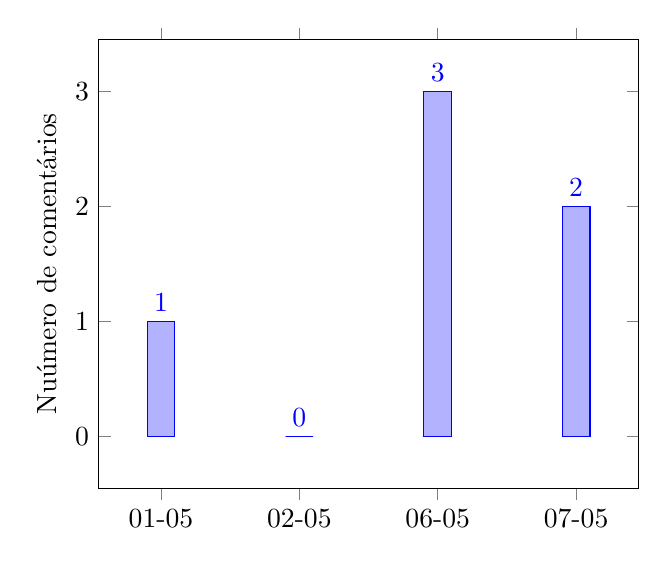
\begin{tikzpicture}
        \begin{axis}[
            ybar,
            enlargelimits=0.15,
            legend style={at={(0.5,-0.15)},
                anchor=north,legend columns=-1},
            ylabel={Nuúmero de comentários},
            symbolic x coords={01-05, 02-05, 06-05, 07-05},
            xtick=data,
            nodes near coords,
            nodes near coords align={vertical},
            ]
        \addplot coordinates {(01-05, 1) (02-05, 0) (06-05, 3) (07-05, 2)};
        \end{axis}
    \end{tikzpicture}
\end{figure}

\section{Utilizador que deram o maior número de \textit{likes} às publicações de um outro}

Amigos chegados normalmente irão dar gosto na publicações um do outro. \par

Deste modo, seria possível tentar prever quem seria o amigo mais próximo de um utilizador ao analisar quem foi aquele que deixou o maior número total de \textit{likes} nas suas publicações, residindo aí o intuito desta interrogação.

\section{Maior "influenciador" da rede social}

Esta interrogação permite obter uma estimativa do maior "influenciador" da nossa rede social. \par

Para o cálculo desta estimativa realizou-se a média aritmética entre o número total de amigos do utilizador, a quantidade de eventos passados a que foi ou eventos futuros que planeia ir e o número de comentários de outros utilizadores feitos nas suas publicações. \par 

Deste modo, é obtido uma pontuação para cada utilizador que classifica o seu grau de influência. Quem possuir o maior \textit{score} será considerado o maior influenciador do FEUPBook.

\begin{equation*}
    score = \frac{N_{amigos} + N_{eventos} + N_{comentarios}}{3}
\end{equation*}

\section{Grau de separação entre cada par de utilizadores}
    
Existe uma teoria, denominada de teoria dos seis graus de separação, que afirma que são necessários no máximo seis laços de amizade para que duas pessoas quaisquer estejam ligadas. \par

Como tal, realizámos esse estudo na nossa rede social e calculámos a quantos amigos uma pessoa estava da outra (gau de separação) para cada utilizador da rede social através desta interrogação.


\begin{figure}[H]
    \centering
    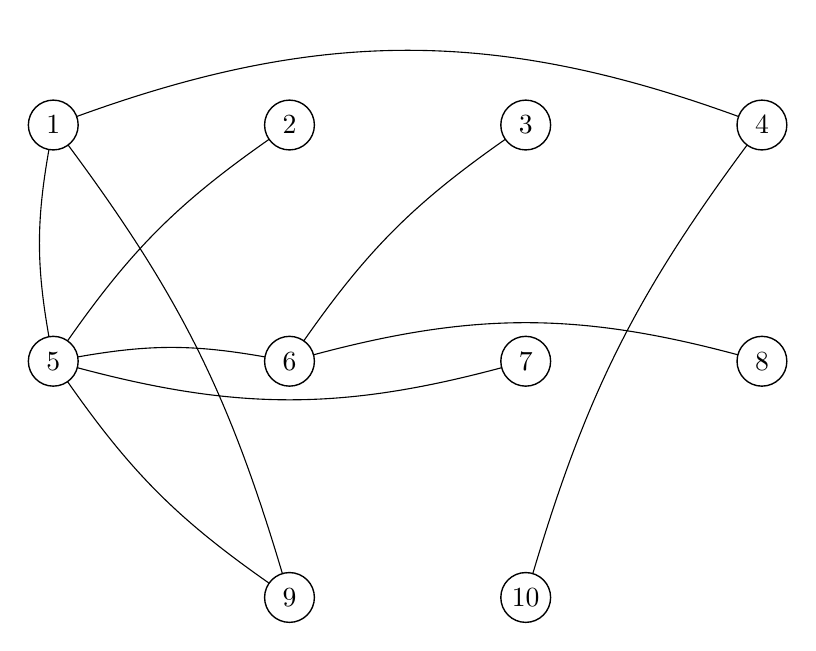
\begin{tikzpicture}
        \SetGraphUnit{3}

        \Vertex{1}

        \EA(1){2}
        \EA(2){3}
        \EA(3){4}
        
        \SO(1){5}
        \SO(2){6}
        \SO(3){7}
        \SO(4){8}
        \SO(6){9}
        \SO(7){10}

        \path [-] (1) edge[bend left=20] (4);
        \path [-] (1) edge[bend right=10] (5);
        \path [-] (1) edge[bend left=10] (9);

        \path [-] (2) edge[bend right=10] (5);
        
        \path [-] (3) edge[bend right=10] (6);

        \path [-] (4) edge[bend right=10] (10);

        \path [-] (5) edge[bend left=10] (6);
        \path [-] (5) edge[bend right=15] (7);
        \path [-] (5) edge[bend right=10] (9);

        \path [-] (6) edge[bend left=15] (8);
    \end{tikzpicture}
\end{figure}

\chapter{Gatilhos}

\section{Limite de amigos}

Este \textit{trigger} permite manter um número de amigos limitados na rede social, ou seja, quando há uma inserção na tabela Friendship se o utilizador já tiver o número máximo de amigos a inserção é parada.

\section{Participação num evento}

Este \textit{trigger} faz com que quando um utilizador pressiona um botão a dizer que vai ou foi a um certo evento(há uma inserção na tabela \textit{EventParticipant}) este faz um post no perfil do utilizador. O conteúdo deste post pode ser "I went to (\textit{event name})" se o evento já tiver acontecido e "I will participate in (\textit{event name})" se ainda for acontecer.

\section{Novo administrador de um grupo}

Este \textit{trigger} faz com que quando um utilizador é convidado para ser administrador de um grupo ao qual não pertence este é automaticamente adicionado e o administrador atual perde o cargo e passa a ser membro.

\end{document}
